\documentclass{ximera}
\title{Written Homework}
\begin{document}
\begin{abstract}
\end{abstract}
\maketitle

\section{Written Homework}

\begin{problem}
Consider the surface described by $(r-3)^2 +z^2 = 1$ in cylindrical coordinates, with the restriction $r\geq 0$.
\begin{enumerate}
\item Sketch the intersection of the surface with the half-plane $\theta = 0$.
\item Sketch the intersection of the surface with the half-plane $\theta = \frac{\pi}{2}$.
\item Sketch the intersection of the surface with the plane $z = 0$. 
\item Sketch the surface.
\end{enumerate}
\end{problem}

\begin{problem}
Sketch the region in $\mathbb{R}^3$ with cylindrical coordinates satisfying the inequality
\[
r\leq z \leq 4-2r
\]
\end{problem}

\begin{problem}
\begin{enumerate}
\item Given a function $f$, consider the graphs of the equations $r = f(\theta)$ and $r = 2f(\theta)$, in polar coordinates. How are these graphs related?
\item Given a function $f$, consider the graphs of the equations $\rho = f(\theta, \phi)$ and $\rho = 2f(\theta, \phi)$, in spherical coordinates. How are these graphs related?
\item Given a function $f$, consider the graphs of the equations $r = f(\theta)$ and $r = -f(\theta)$, in polar coordinates. How are these graphs related?
\item Given a function $f$, consider the graphs of the equations $\rho = f(\theta, \phi)$ and $\rho = -f(\theta, \phi)$, in spherical coordinates. How are these graphs related?
\end{enumerate}
\end{problem}

\section{Professional Problem}

\begin{problem}
Consider the solid in $\mathbb{R}^3$ shown below.

\begin{image}
\begin{tikzpicture}
\node[inner sep=0pt] at (0,0)
    {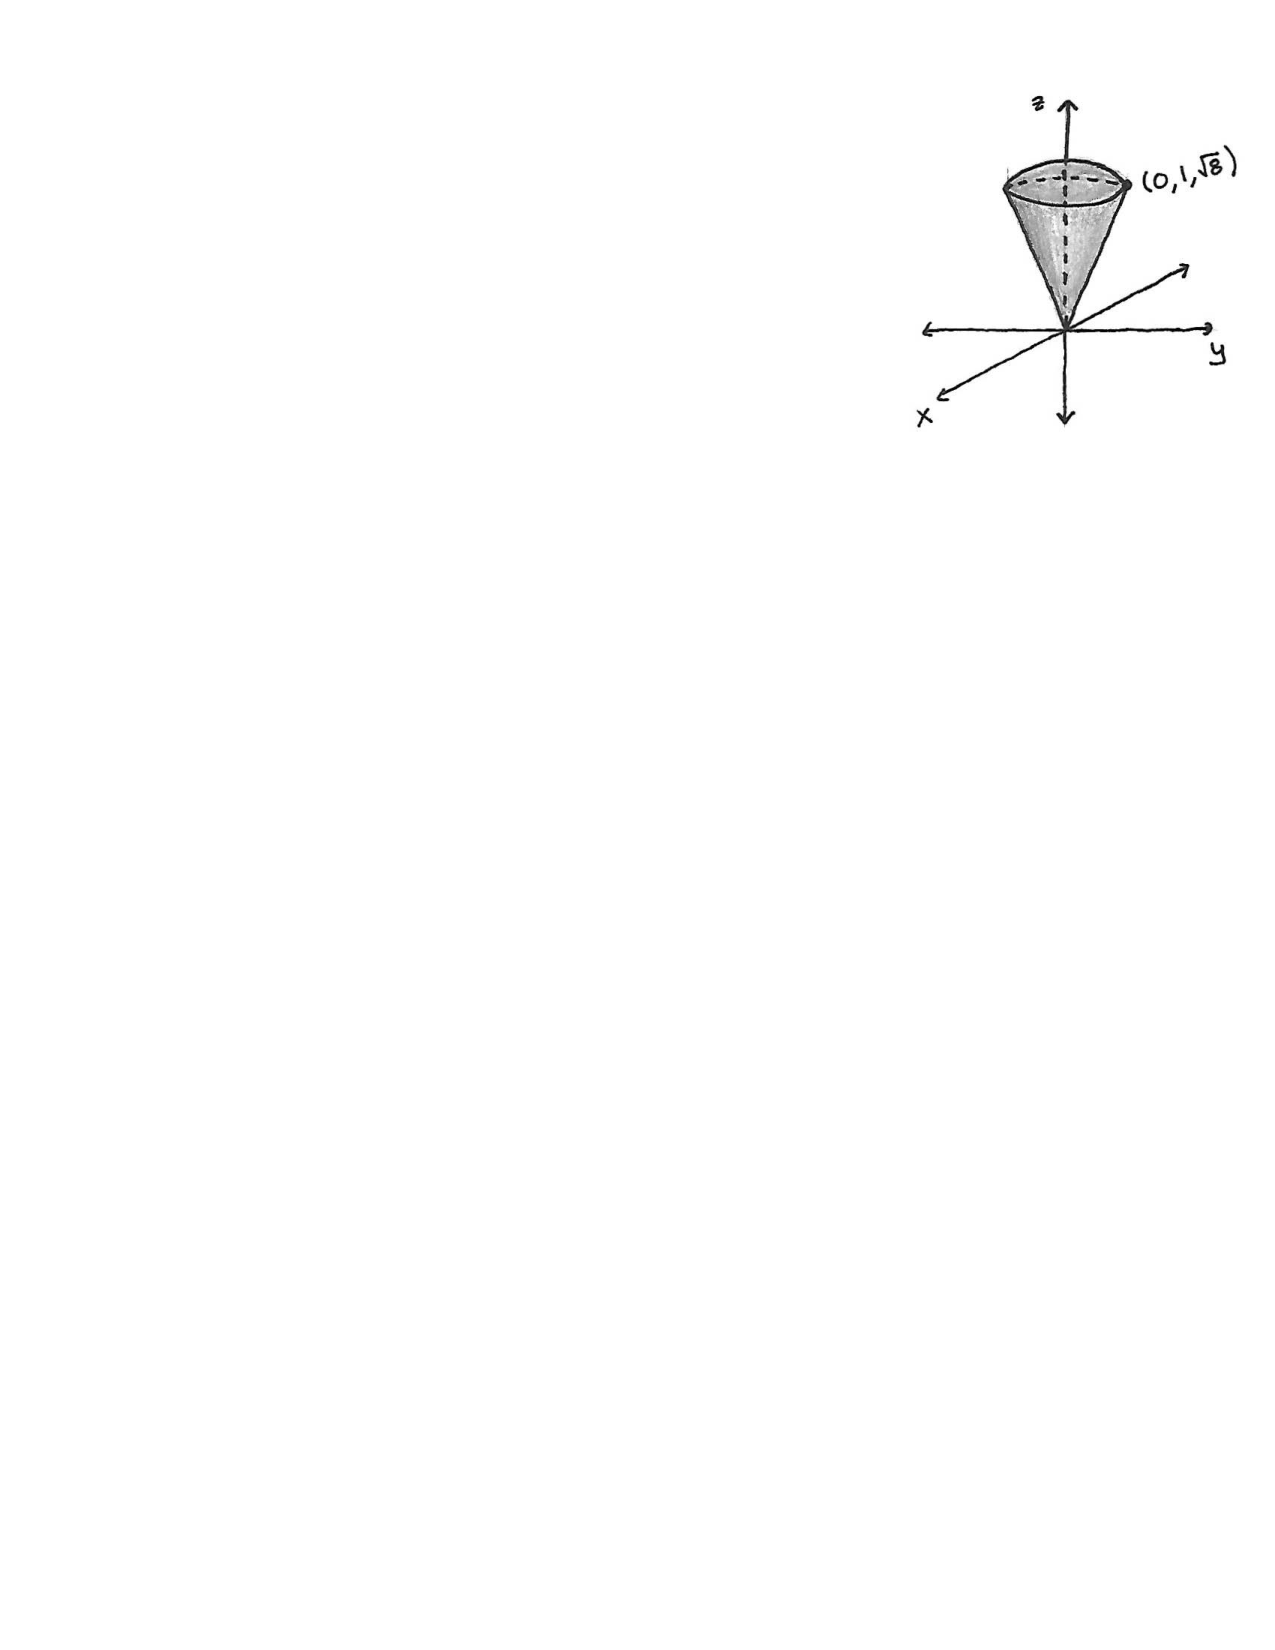
\includegraphics{ice_cream_pp}};
\end{tikzpicture}
\end{image}

\begin{enumerate}
\item Describe the solid using spherical coordinates.
\item Describe the solid using cylindrical coordinates.
\end{enumerate}

Your solution should be professionally written, following the instructions given in class and in the Professional Problem information sheet. In particular, be sure to focus on the following (which is \emph{not} an exhaustive list!):
\begin{itemize}
	\item \textbf{Structure:} State your solution in brief, and then concisely explain why it is correct.
	\item \textbf{Formatting:} Be sure to follow the formatting requirements on Moodle. Staple the checklist to your problem, it will be used as part of your assessment.
	\item \textbf{Figures:} Include a clearly labeled figure for each part of the problem. The labels should help to demonstrate why your solution is correct. Label everything which is necessary, and nothing which is not. Refer to the figure in your solution as necessary.
	\item \textbf{\LaTeX:} (optional) If you wish you type your solution in \LaTeX, use the tex file on Moodle.
\end{itemize}
\end{problem}

\end{document}